\begin{frame}
  \frametitle{The variance of a data set}
  %% \framesubtitle{}

  \begin{itemize}
  \item Rationale: find the dimensions that give the best (statistical)
    explanation for the \h{variance} (or ``spread'') of the data
  \item Definition of the variance of a set of vectors
    \begin{itemize}
    \item[\hand] you remember the equations for one-dimensional data, right?
    \end{itemize}
    \ungap\pause
    \begin{align*}
      \sigma^2 &= \frac{1}{k-1} \sum_{i=1}^k \norm{\vx[i] - \vmu}^2 \\
      \vmu &= \frac{1}{k} \sum_{i=1}^k \vx[i]
    \end{align*}
  \item Easier to calculate if we \h{center} the data so that $\vmu = \vnull$
  \end{itemize}
\end{frame}

\begin{frame}[c]
  \frametitle{Centering the data set}
  %% \framesubtitle{}

  \begin{columns}[c]
    \begin{column}{40mm}
      \begin{itemize}
      \item \h<beamer:1| handout:1>{Uncentered\\ data set}%
        \gap
      \item \h<beamer:2| handout:2>{Centered\\ data set}%
        \gap
      \item \h<beamer:3| handout:3>{Variance of\\ centered data}%
        \gap
      \end{itemize}
      \visible<beamer:3| handout:3>{%
        \[
        \sigma^2 = \tfrac{1}{k-1} \sum_{i=1}^k \norm{\vx[i]}^2
        \]
      }
    \end{column}
    \begin{column}{60mm}
      \only<beamer:1| handout:1>{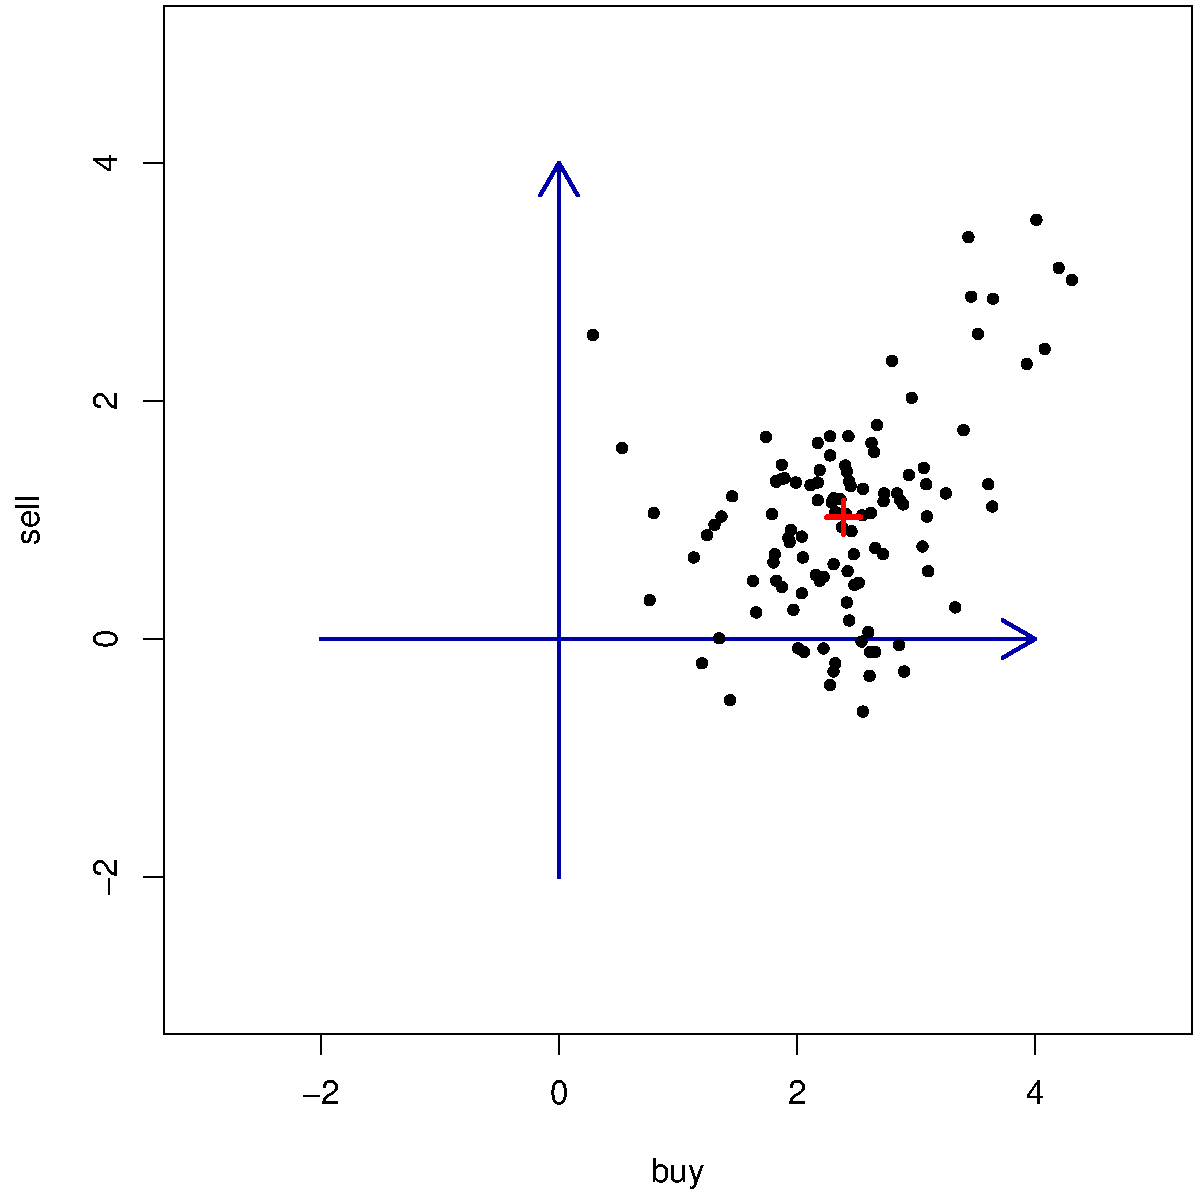
\includegraphics[width=6cm]{img/3_buy_sell_uncentered}}%
      \only<beamer:2| handout:2>{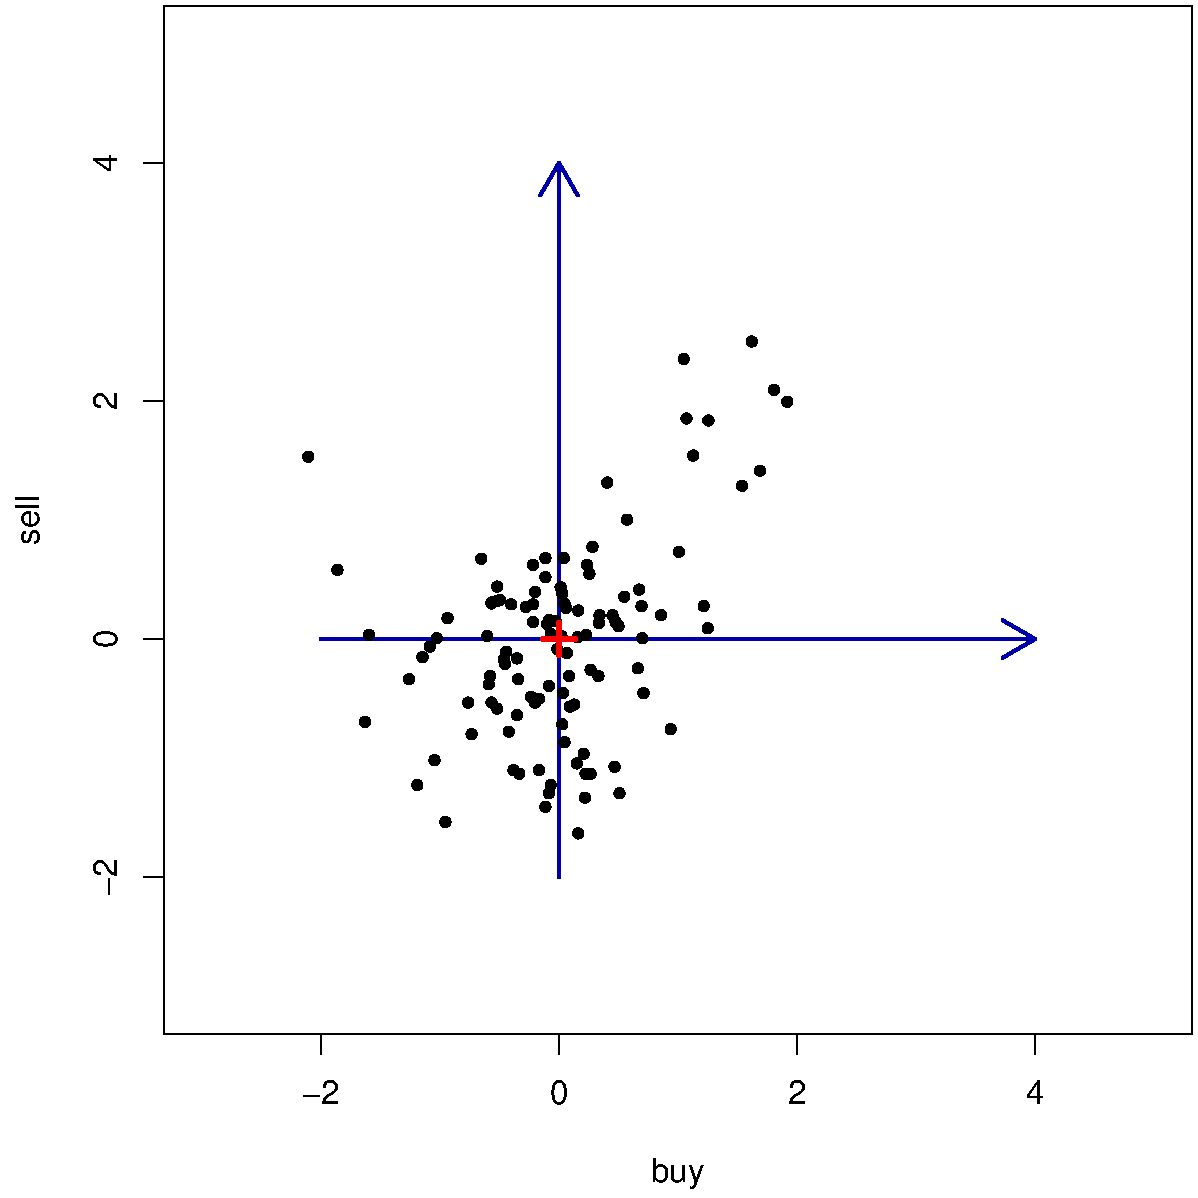
\includegraphics[width=6cm]{img/3_buy_sell_centered}}%
      \only<beamer:3| handout:3>{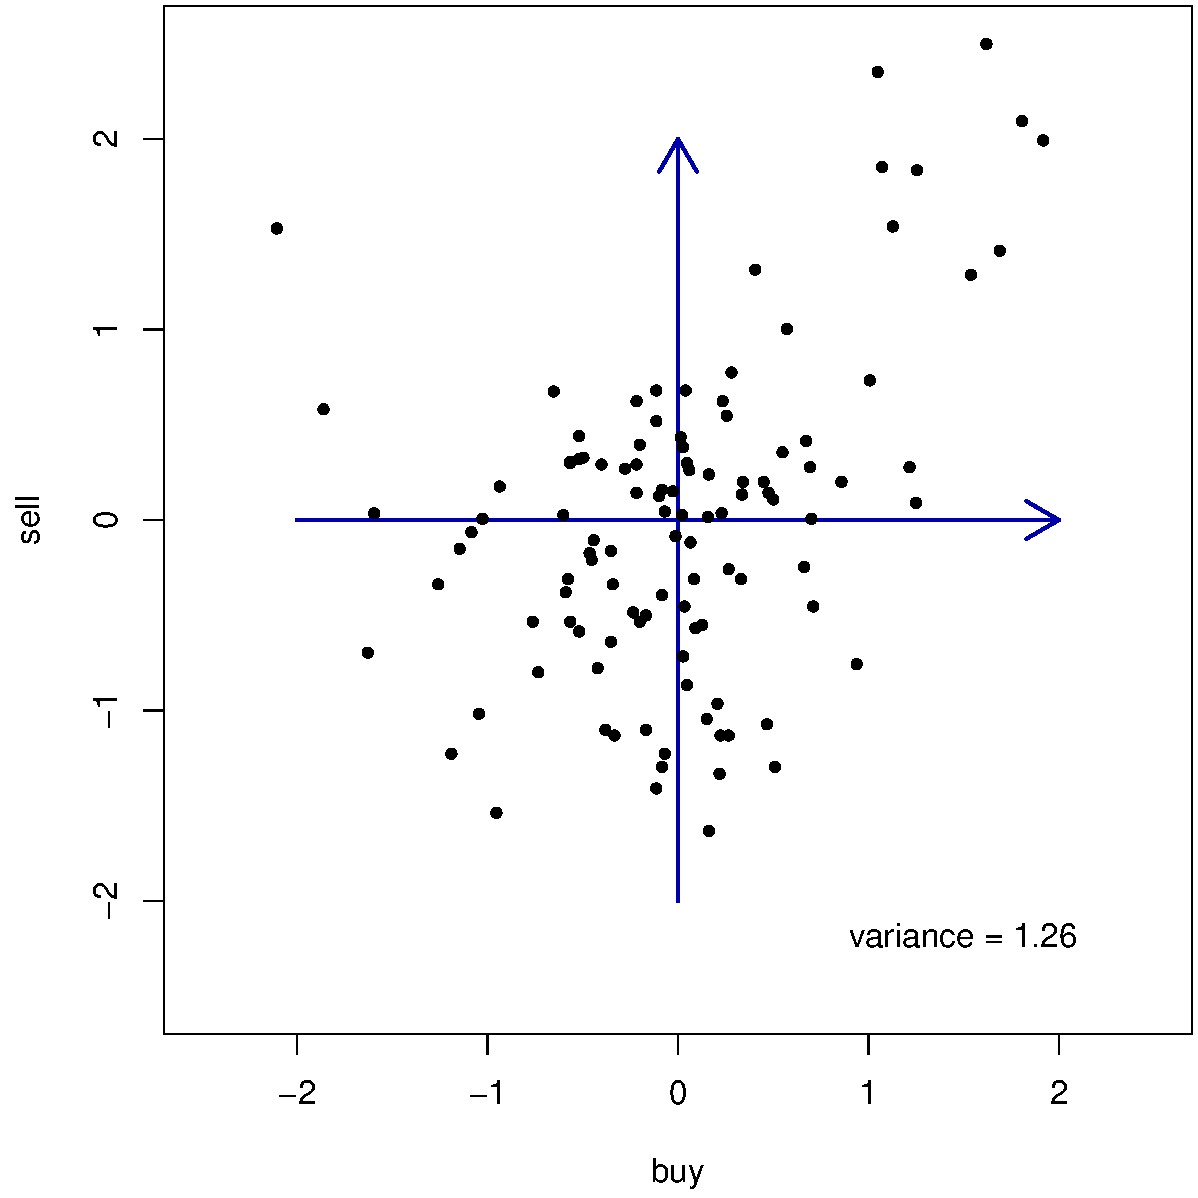
\includegraphics[width=6cm]{img/3_buy_sell_variance}}%
    \end{column}
  \end{columns}
\end{frame}

%%% Local Variables: 
%%% mode: latex
%%% TeX-master: "../../workspace"
%%% End: 
